%%%%%%%%%%%%%%%%%%%%%%%%%%%%% Define Article %%%%%%%%%%%%%%%%%%%%%%%%%%%%%%%%%%
\documentclass{article}
%%%%%%%%%%%%%%%%%%%%%%%%%%%%%%%%%%%%%%%%%%%%%%%%%%%%%%%%%%%%%%%%%%%%%%%%%%%%%%%

%%%%%%%%%%%%%%%%%%%%%%%%%%%%% Using Packages %%%%%%%%%%%%%%%%%%%%%%%%%%%%%%%%%%
\usepackage{geometry}
\usepackage{graphicx}
\usepackage{amssymb}
\usepackage{amsmath}
\usepackage{amsthm}
\usepackage{empheq}
\usepackage{mdframed}
\usepackage{booktabs}
\usepackage{lipsum}
\usepackage{listings}
\usepackage{graphicx}
\usepackage{color}
\usepackage{psfrag}
\usepackage{pgfplots}
\usepackage{bm}
\usepackage{xcolor}
%%%%%%%%%%%%%%%%%%%%%%%%%%%%%%%%%%%%%%%%%%%%%%%%%%%%%%%%%%%%%%%%%%%%%%%%%%%%%%%

% Other Settings

\lstset{
  language=R,
  basicstyle=\ttfamily\small,
  keywordstyle=\color{blue}\bfseries,
  commentstyle=\color{green!50!black},
  stringstyle=\color{orange},
  numbers=left,
  numberstyle=\tiny,
  stepnumber=1,
  numbersep=5pt,
  backgroundcolor=\color{gray!10},
  frame=single,
  breaklines=true,
  captionpos=b,
  tabsize=2
}

%%%%%%%%%%%%%%%%%%%%%%%%%% Page Setting %%%%%%%%%%%%%%%%%%%%%%%%%%%%%%%%%%%%%%%
\geometry{a4paper}

%%%%%%%%%%%%%%%%%%%%%%%%%% Define some useful colors %%%%%%%%%%%%%%%%%%%%%%%%%%
\definecolor{ocre}{RGB}{243,102,25}
\definecolor{mygray}{RGB}{243,243,244}
\definecolor{deepGreen}{RGB}{26,111,0}
\definecolor{shallowGreen}{RGB}{235,255,255}
\definecolor{deepBlue}{RGB}{61,124,222}
\definecolor{shallowBlue}{RGB}{235,249,255}
%%%%%%%%%%%%%%%%%%%%%%%%%%%%%%%%%%%%%%%%%%%%%%%%%%%%%%%%%%%%%%%%%%%%%%%%%%%%%%%

%%%%%%%%%%%%%%%%%%%%%%%%%% Define an orangebox command %%%%%%%%%%%%%%%%%%%%%%%%
\newcommand\orangebox[1]{\fcolorbox{ocre}{mygray}{\hspace{1em}#1\hspace{1em}}}
%%%%%%%%%%%%%%%%%%%%%%%%%%%%%%%%%%%%%%%%%%%%%%%%%%%%%%%%%%%%%%%%%%%%%%%%%%%%%%%

%%%%%%%%%%%%%%%%%%%%%%%%%%%% English Environments %%%%%%%%%%%%%%%%%%%%%%%%%%%%%
\newtheoremstyle{mytheoremstyle}{3pt}{3pt}{\normalfont}{0cm}{\rmfamily\bfseries}{}{1em}{{\color{black}\thmname{#1}~\thmnumber{#2}}\thmnote{\,--\,#3}}
\newtheoremstyle{myproblemstyle}{3pt}{3pt}{\normalfont}{0cm}{\rmfamily\bfseries}{}{1em}{{\color{black}\thmname{#1}~\thmnumber{#2}}\thmnote{\,--\,#3}}
\theoremstyle{mytheoremstyle}
\newmdtheoremenv[linewidth=1pt,backgroundcolor=shallowGreen,linecolor=deepGreen,leftmargin=0pt,innerleftmargin=20pt,innerrightmargin=20pt,]{theorem}{Theorem}[section]
\theoremstyle{mytheoremstyle}
\newmdtheoremenv[linewidth=1pt,backgroundcolor=shallowBlue,linecolor=deepBlue,leftmargin=0pt,innerleftmargin=20pt,innerrightmargin=20pt,]{definition}{Definition}[section]
\theoremstyle{myproblemstyle}
\newmdtheoremenv[linecolor=black,leftmargin=0pt,innerleftmargin=10pt,innerrightmargin=10pt,]{problem}{Problem}[section]
%%%%%%%%%%%%%%%%%%%%%%%%%%%%%%%%%%%%%%%%%%%%%%%%%%%%%%%%%%%%%%%%%%%%%%%%%%%%%%%

%%%%%%%%%%%%%%%%%%%%%%%%%%%%%%% Plotting Settings %%%%%%%%%%%%%%%%%%%%%%%%%%%%%
\usepgfplotslibrary{colorbrewer}
\pgfplotsset{width=8cm,compat=1.9}
%%%%%%%%%%%%%%%%%%%%%%%%%%%%%%%%%%%%%%%%%%%%%%%%%%%%%%%%%%%%%%%%%%%%%%%%%%%%%%%

%%%%%%%%%%%%%%%%%%%%%%%%%%%%%%% Title & Author %%%%%%%%%%%%%%%%%%%%%%%%%%%%%%%%
\title{Math 133 - Group Work 2}
\author{Pranav Jayakumar}
%%%%%%%%%%%%%%%%%%%%%%%%%%%%%%%%%%%%%%%%%%%%%%%%%%%%%%%%%%%%%%%%%%%%%%%%%%%%%%%

\begin{document}
    \maketitle
    \begin{abstract}
      In this assignment, we compare the different predictors of sales (TV, radio, newspaper). 
    \end{abstract}

    \section{Data Analysis}
    \vspace{0.1in}
    \subsection{Fitting Linear Models}

    We will first create three linear models for the three predictors of sales. We will use a 80-20 training-testing split. We initialize a seed of \verb|123| to maintain reproducibility.
    \vspace{0.1in}
    \begin{lstlisting}
    fit_linear_model <- function(y, x, raw_data) {

      # train test split
      n <- nrow(raw_data)
      trainIndex <- sample(n, round(0.8 * n, 0))
      train <- raw_data[trainIndex, ]
      test <- raw_data[-trainIndex, ]
  
      # construct formula
      formula <- as.formula(paste(y, "~", x))
  
      # fit model
      model <- lm(formula, data = train)
  
      # predict on testing data
      y_test <- test[[y]]
      y_hat <- predict(model, newdata = test)
  
      # analyze accuracy
      SSE <- sum((y_test - y_hat)^2)
      MSE <- SSE / nrow(test)  
      RMSE <- sqrt(MSE)
      SST <- sum((y_test - mean(y_test))^2)
      R2 <- 1 - SSE / SST
  
      return(list(SSE = SSE, MSE = MSE, RMSE = RMSE, SST = SST, R2 = R2))
    }
    \end{lstlisting}

    We observe that for the linear model \verb|sales~TV|, $R^2 = 0.6053$. For the linear model \verb|sales~radio|, we observe that $R^2 = 0.2692$. 
    For the linear model \verb|sales~newspaper|, we observe that $R^2 = -0.0693$. 
    \vspace{0.1in}
    \subsection{Interpretation of Results}
    Based on the results from the $R^2$ tests, we determine \verb|TV| to be the best predictor of \verb|sales|.
    \vspace{0.1in}
    \subsection{Visualization}
    Below is a scatterplot denoting sales vs $x$ where $x$ is the \verb|TV| predictor.
    \vspace{0.1in}
    \begin{figure}[h]
      \begin{center}
        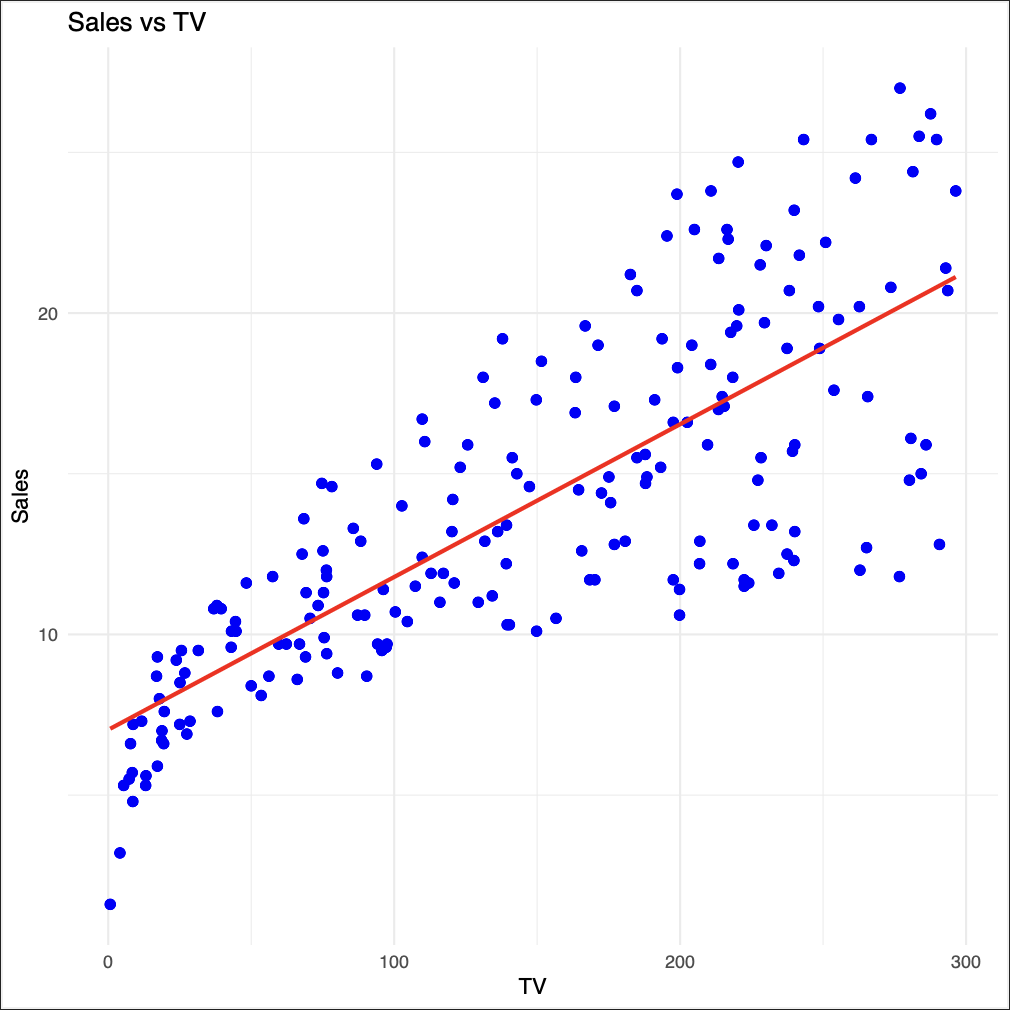
\includegraphics[width=0.95\textwidth]{sales_vs_tv.png}
      \end{center}
    \end{figure}
    \section{Complete R Code}
    \begin{lstlisting}
#!/usr/bin/env Rscript
library(ggplot2)

set.seed(123)

fit_linear_model <- function(y, x, raw_data) {

  # train test split
  n <- nrow(raw_data)
  trainIndex <- sample(n, round(0.8 * n, 0))
  train <- raw_data[trainIndex, ]
  test <- raw_data[-trainIndex, ]
  
  # construct formula
  formula <- as.formula(paste(y, "~", x))
  
  # fit model
  model <- lm(formula, data = train)
  
  # predict on testing data
  y_test <- test[[y]]
  y_hat <- predict(model, newdata = test)
  
  # analyze accuracy
  SSE <- sum((y_test - y_hat)^2)
  MSE <- SSE / nrow(test)  
  RMSE <- sqrt(MSE)
  SST <- sum((y_test - mean(y_test))^2)
  R2 <- 1 - SSE / SST
  
  return(list(SSE = SSE, MSE = MSE, RMSE = RMSE, SST = SST, R2 = R2))
}

main <- function() {
   # Load data
  advertising <- read.csv("../../data/Advertising.csv")
  
  # Define predictors
  predictors <- c("TV", "radio", "newspaper")
  results <- list()
  
  # Iterate over predictors
  for (predictor in predictors) {
    if (!predictor %in% colnames(advertising)) {
      cat("\nWarning: Predictor", predictor, "not found in dataset. Skipping...\n")
      next
    }
    
    cat("\nLinear model for sales ~", predictor, "\n")
    result <- fit_linear_model("sales", predictor, advertising)
    
    # Store results for later comparison
    results[[predictor]] <- result
    
    # Format and print results
    formatted_results <- lapply(result[1:5], function(x) format(round(x, 4), nsmall = 4))
    print(formatted_results)
  }
  
  # Determine the best predictor (highest R^2)
  best_predictor <- names(results)[which.max(sapply(results, function(r) r$R2))]
  cat("\nBest predictor based on R^2:", best_predictor, "\n")
  
  # Create scatterplot for the best predictor
  ggplot(advertising, aes_string(x = best_predictor, y = "sales")) +
    geom_point(color = "blue", size = 2) +
    geom_smooth(method = "lm", color = "red", se = FALSE) +
    ggtitle(paste("Sales vs", best_predictor)) +
    xlab(best_predictor) +
    ylab("Sales") +
    theme_minimal()
}

# Run the script if executed directly
if (interactive() || identical(Sys.getenv("R_SCRIPT"), "")) {
  main()
  \end{lstlisting}

\end{document}
